 \begin{center}\begin{large} Homework Problems 4
 \end{large}\end{center}
 \bigskip

\begin{problem}[2 points]
   Find, if exists, the limit of the sequence, as $n\to\infty$:

    \begin{enumerate}
        \item[a) ] $\dfrac{3-n}{2}$,
        
        \item[b) ] $\dfrac{3-n^2}{2+n^3}$,
        
        \item[c) ] $\dfrac{(n+1)^2(n+2)^3}{n^6}$,
        
        \item[d) ] $\dfrac{(n+1)^2(n+2)^3}{n^5}$,
        
        \item[e) ] $1^n$,

        \item[f) ] $(-1)^n$,

        \item[g) ] $\left(\dfrac{1}{0.99}\right)^n$,

        \item[h) ] $\sin {n}$,

        \item[i) ] $\dfrac{\sin {n}}{n}$.

    \end{enumerate}
    Which of the sequences above are convergent?

\end{problem}

\bigskip

\begin{problem}[2 points]
Find the value of $c$, if exists, such that the following function 
$f
(
x
)$ is continuous at 
$2$.
    \begin{enumerate}
    \item[a) ] $
f(x)=\begin{cases} 3x-5,& \text{if \(x\neq 2\)} \\  x^2+c,& \text{if \(x\ge2\)} \end{cases} $

        \item[b) ] $
f(x)=\begin{cases} x^3+1,& \text{if } x<2 \\  cx^2,& \text{if \(x\ge2\)} \end{cases} $ 
        
        \item[c) ] $
f(x)=\begin{cases} -7,& \text{if } x<2 \\ c,& \text{if } x=2 \\  4+3\sin(\pi x),& \text{if \(x>2\)} \end{cases} $
\bigskip
        
        \item[d) ] $
f(x)=\begin{cases} {\dfrac{x^2-x-2}{x-2}},& \text{if \(x\neq 2\)} \\  c,& \text{if \(x<2\)} \end{cases} $
        
    \end{enumerate}
\end{problem}
\bigskip


\begin{problem}[2 points]
Find the derivatives of the following functions:
    \begin{enumerate}
    \item[a) ] $10000$,

        \item[b) ] $2x^2-7x+1$,
        
        \item[c) ] $2\sin x \cdot e^x$,
        
        \item[d) ] $e^{x^2}$,
        \item[e) ] $x^2\ln x$,
        \item[f) ] $\dfrac{x^2}{x^3}$,
        \item[g) ] $\dfrac{x^2}{x^3+1}$,
        \item[h) ] $\sin(\cos x)$.
    \end{enumerate}
\end{problem}
\bigskip


\begin{problem}[3 points]
Find the points of local extremum of $f(x)$ on the given set:
    \begin{enumerate}
    \item[a) ] $f(x)=5x-x^2,\: x\in[2,12]$,
    \item[b) ] $f(x)=3x+1, \: x\in[-5, 5]$,
    \item[c) ] $f(x)=\dfrac{x-1}{x^2+1},\: x\in\R$,
    \item[d) ] $f(x)=\dfrac{x^3}{e^x},\: x\in\R$,
        \item[e) ] $f(x)=\cos x-\sin x,\: x\in[0,\pi]$.
        
    \end{enumerate}
\end{problem}
\bigskip


\begin{problem}[1 point]
Calculate $\displaystyle \int f(x)\, dx$:
    \begin{enumerate}
        \item[a) ] $f(x)=x^3$,
        \item[b) ] $f(x)=7x^4-3$,
        \item[c) ] $f(x)=\cos4x$,
    \end{enumerate}
\end{problem}


\bigskip

\begin{problem}[\textbf{optional, not graded}]
Match the graphs 1-4 to functions i-iv: 
\\~\\
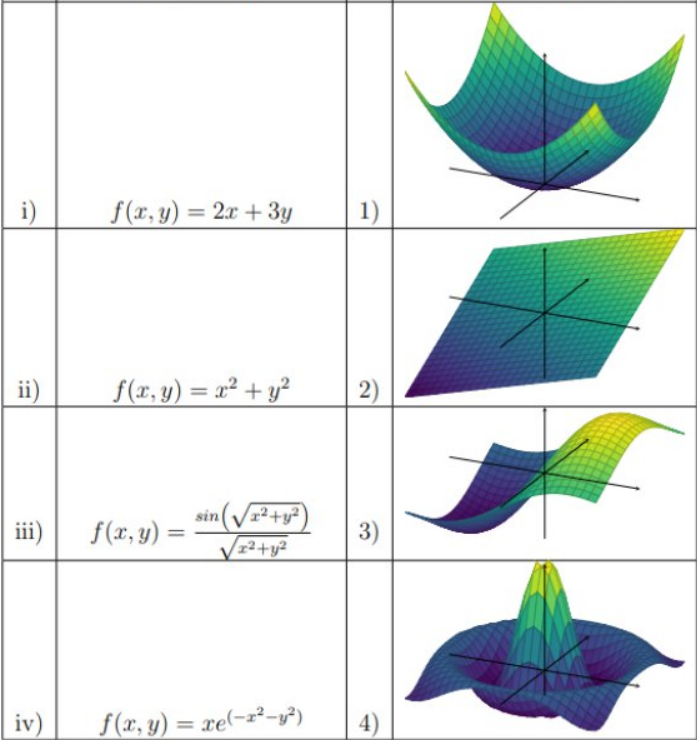
\includegraphics[width=0.7\linewidth]{figs/f(x,y) functions.png}
\\~\\
\end{problem}